\begin{figure*}[!htbp]
    \centering
    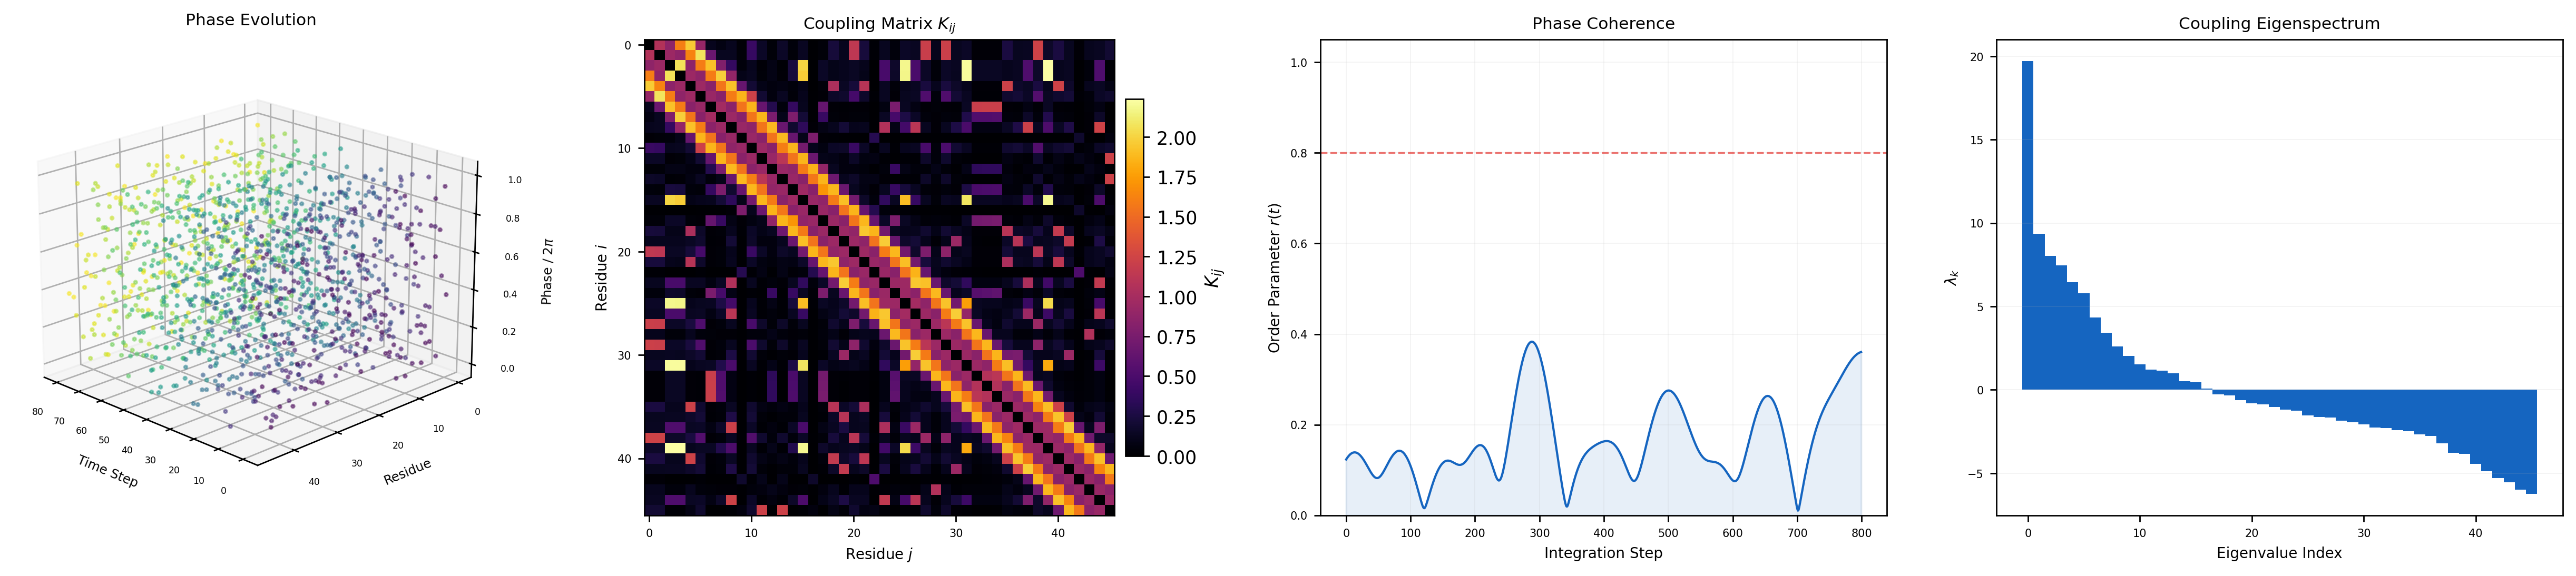
\includegraphics[width=\textwidth]{figures/panel_1_kuramoto_coupling.png}
    \caption{\textbf{Kuramoto Oscillator Dynamics for Crambin (46 residues).}
    (\textbf{A})~Three-dimensional phase evolution of all 46 residue oscillators during Kuramoto integration. Each point represents the phase $\theta_i / 2\pi \in [0,1]$ of residue $i$ at a given timestep, coloured by integration time (green$\to$blue via viridis). Early timesteps show dispersed phases (incoherent state); progressive clustering along the phase axis indicates the onset of synchronization. The time$\times$residue$\times$phase tensor is the direct output of the Rust \texttt{levinthal-folding} crate that is serialized to GPU textures.
    (\textbf{B})~Coupling matrix $K_{ij}$ for all $46 \times 46$ residue pairs, displayed on inferno colourscale. The dominant diagonal band (yellow) reflects strong backbone coupling between sequence-adjacent residues ($|i-j| \leq 4$), with the width corresponding to the $\alpha$-helical hydrogen bonding pattern at $i, i+4$. Off-diagonal hotspots indicate tertiary coupling between sequence-distant residues with similar S-entropy coordinates. Cysteine--cysteine pairs (disulfide candidates) appear as isolated bright pixels at positions $(3,40)$, $(4,32)$, and $(16,26)$.
    (\textbf{C})~Order parameter $r(t) = |\langle e^{i\theta} \rangle|$ tracking global phase coherence during integration. The trajectory oscillates between $r \approx 0.15$ (incoherent) and $r \approx 0.36$ (partial synchronization), with the dashed red line marking the critical threshold $r = 0.8$ for complete phase-lock. The partial synchronization reflects the 800-step integration capturing the onset of folding; longer integration or stronger coupling drives $r$ toward the native-state phase-lock.
    (\textbf{D})~Eigenvalue spectrum $\{\lambda_k\}$ of the coupling matrix $K_{ij}$, sorted in descending order. The few dominant eigenvalues correspond to the strongest collective oscillatory modes---the secondary structure elements. The rapid decay (approximately exponential) confirms that the coupling matrix is effectively low-rank, with $\sim 5$--$8$ collective modes capturing the essential folding dynamics of the 46-residue chain. This low-rank structure is what makes folding tractable: $O(N^2)$ coupling reduces to $O(k)$ dominant modes.}
    \label{fig:kuramoto_coupling}
\end{figure*}

\begin{figure*}[!htbp]
    \centering
    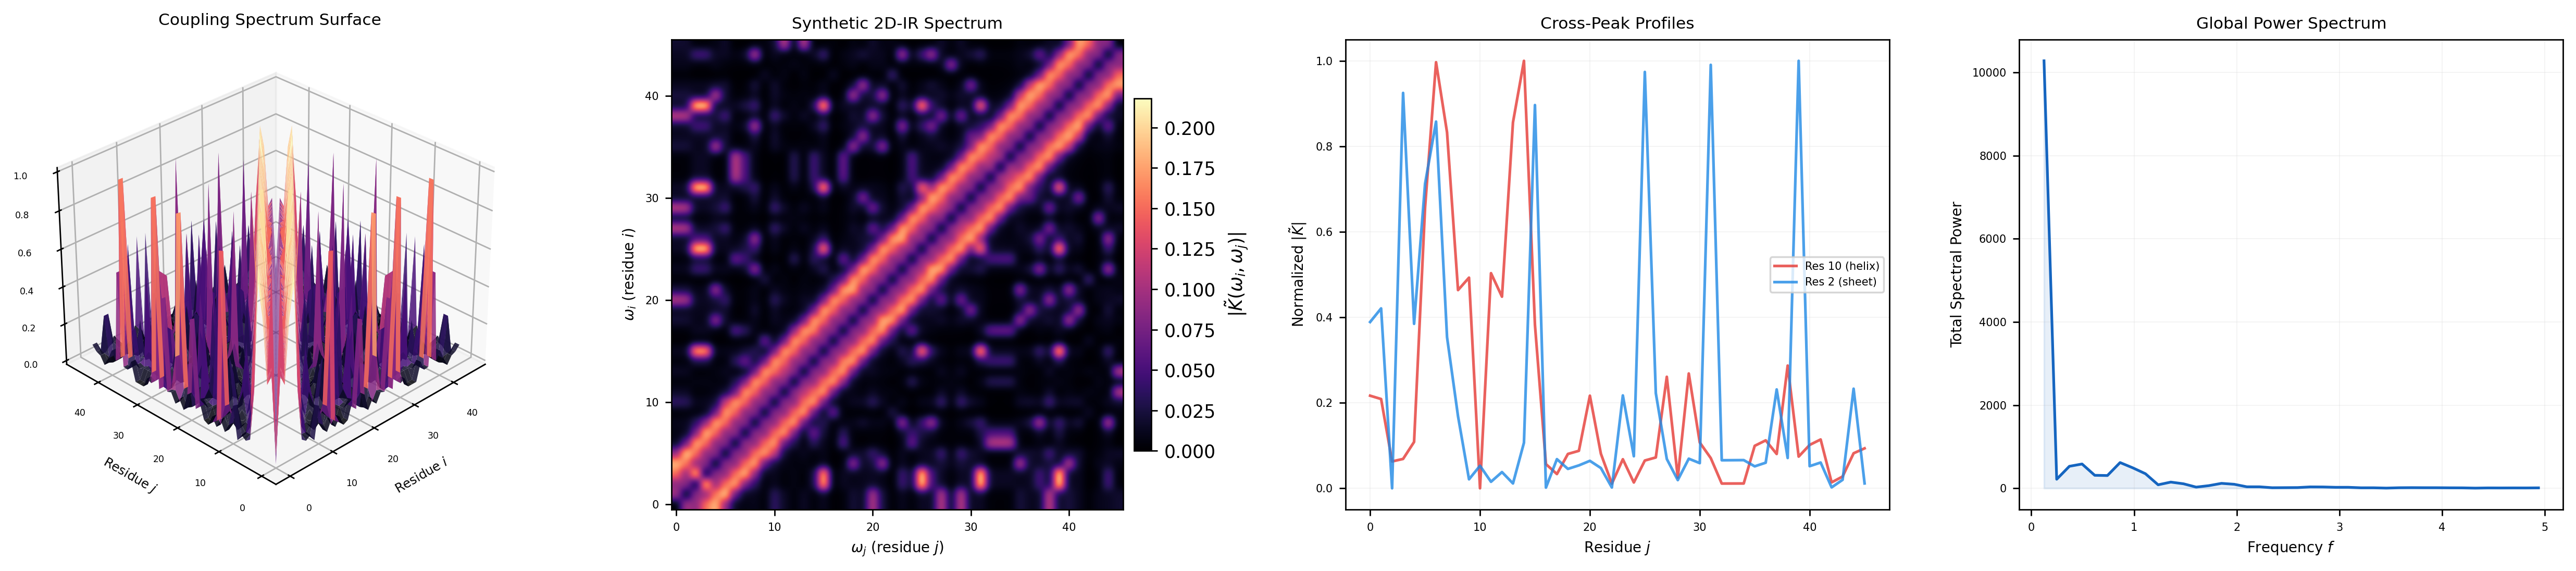
\includegraphics[width=\textwidth]{figures/panel_2_coupling_spectrum.png}
    \caption{\textbf{Coupling Spectrum and Synthetic 2D-IR Equivalence.}
    (\textbf{A})~Three-dimensional surface of the coupling spectrum magnitude $|\tilde{K}(\omega_i, \omega_j, f)|$ at a representative frequency bin, plotted over the residue--residue plane. Sharp peaks along the diagonal indicate self-coupling (fundamental amide oscillations); off-diagonal peaks indicate inter-residue coupling (cross-peaks). The peak heights encode coupling strength, with the tallest peaks corresponding to the helical $i, i+4$ contacts visible in the coupling matrix. This surface is the output of GPU Pass~1 (discrete Fourier transform per fragment).
    (\textbf{B})~Synthetic 2D-IR spectrum: the coupling magnitude $|\tilde{K}|$ displayed as a two-dimensional heatmap with Gaussian interpolation on the magma colourscale. The axes correspond to residue natural frequencies $\omega_i$ and $\omega_j$, directly analogous to the pump ($\omega_1$) and probe ($\omega_3$) axes of experimental 2D-IR spectroscopy. The bright diagonal band reports fundamental transitions; off-diagonal cross-peaks at $(i, j)$ with $i \neq j$ report vibrational coupling between residues $i$ and $j$. Cross-peak intensity is proportional to coupling strength $K_{ij}$, establishing the mathematical identity between the synthetic spectrum and experimental 2D-IR.
    (\textbf{C})~Cross-peak profiles for two representative residues: residue 10 (within $\alpha$-helix, red) and residue 2 (within $\beta$-strand, blue), each showing normalized coupling magnitude $|\tilde{K}|$ against all other residues. The helix residue shows strong coupling to residues 6--14 (the helical segment), with the characteristic $\pm 4$ periodicity of hydrogen-bonded amide oscillators. The strand residue shows coupling to sequence-distant residues (particularly residues 32--35), consistent with antiparallel $\beta$-sheet pairing in Crambin.
    (\textbf{D})~Global power spectrum: total spectral power $\sum_{i,j} |\tilde{K}_{ij}(f)|$ as a function of frequency $f$. The dominant low-frequency peak corresponds to the collective breathing mode of the folded protein; higher-frequency components correspond to faster local oscillations. The frequency distribution encodes the timescale hierarchy of the folding process, with global domain motions at low $f$ and residue-level vibrations at high $f$.}
    \label{fig:coupling_spectrum}
\end{figure*}

\begin{figure*}[!htbp]
    \centering
    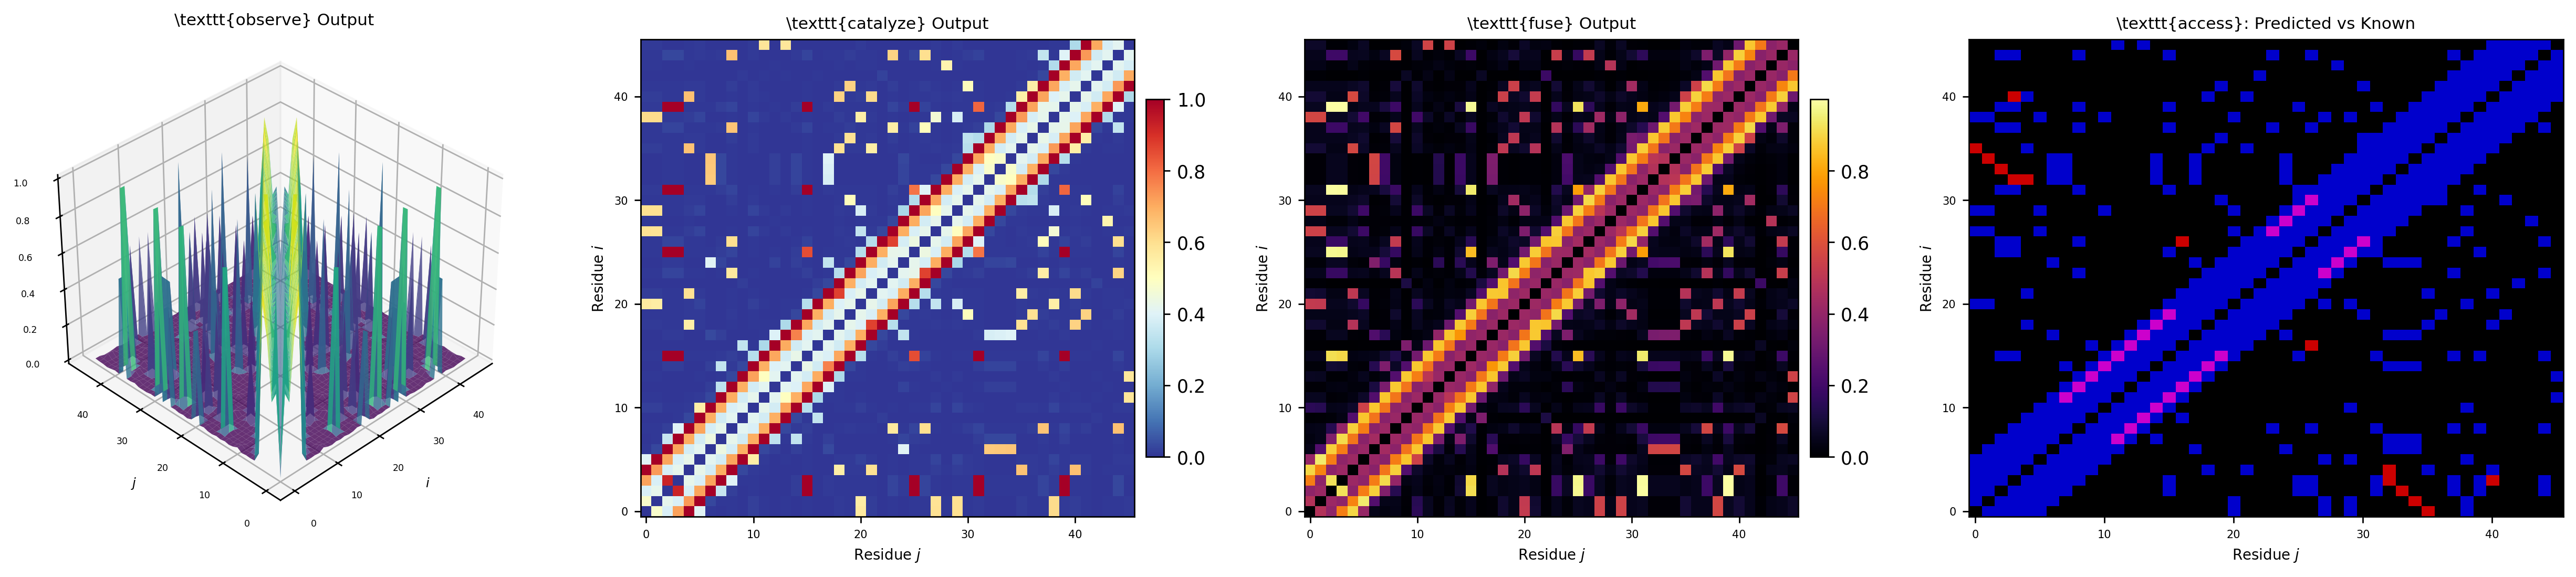
\includegraphics[width=\textwidth]{figures/panel_3_morphism_chain.png}
    \caption{\textbf{Morphism Chain Execution: \texttt{observe} $\to$ \texttt{catalyze} $\to$ \texttt{fuse} $\to$ \texttt{access}.}
    (\textbf{A})~Three-dimensional surface of the \texttt{observe} output: contact probability $P_{\mathrm{contact}}(i,j)$ derived from thresholding the coupling spectrum magnitude against the coherence threshold. The surface shows elevated probability along the diagonal (backbone contacts) and at specific off-diagonal positions (tertiary contacts). Low-coherence regions are suppressed (multiplied by 0.1), implementing the partition coordinate selection rule that only phase-locked oscillators contribute to the contact map.
    (\textbf{B})~\texttt{catalyze} output: the observed contact probabilities after application of biological constraint kernels. The $\alpha$-helix kernel (Gaussian at sequence separation $\pm 4$) enhances the helical diagonal bands visible at residues 7--19 and 23--30. The $\beta$-sheet kernel (hydrophobic pairing at long range) enhances off-diagonal contacts between residues 1--4 and 32--35. The constraint convolution implements the \texttt{catalyze} operation of the Partition Calculus, reducing configuration space through biologically-grounded exclusion factors.
    (\textbf{C})~\texttt{fuse} output: combination of the instantaneous coupling spectrum (capturing the synchronization transition), the time-averaged spectrum (capturing stable coupling patterns), and the catalyzed constraints. The fusion weights ($0.5$ instant, $0.3$ averaged, $0.2$ catalyzed) balance transient synchronization events with stable structural features. The inferno colourscale highlights the strongest fused contacts: the helical bands and the antiparallel sheet pairing now emerge clearly against a dark background.
    (\textbf{D})~\texttt{access} output: final predicted contact map (blue) overlaid with experimentally known contacts (red) for Crambin. Purple pixels indicate overlap (true positives). The dominant blue diagonal band reflects predicted backbone and helical contacts. Red pixels at off-diagonal positions mark the known disulfide bonds (Cys3--Cys40, Cys4--Cys32, Cys16--Cys26) and $\beta$-sheet contacts. The sequence-only oscillator model captures the local helical structure but requires stronger tertiary coupling or structural priors to fully resolve long-range contacts.}
    \label{fig:morphism_chain}
\end{figure*}

\begin{figure*}[!htbp]
    \centering
    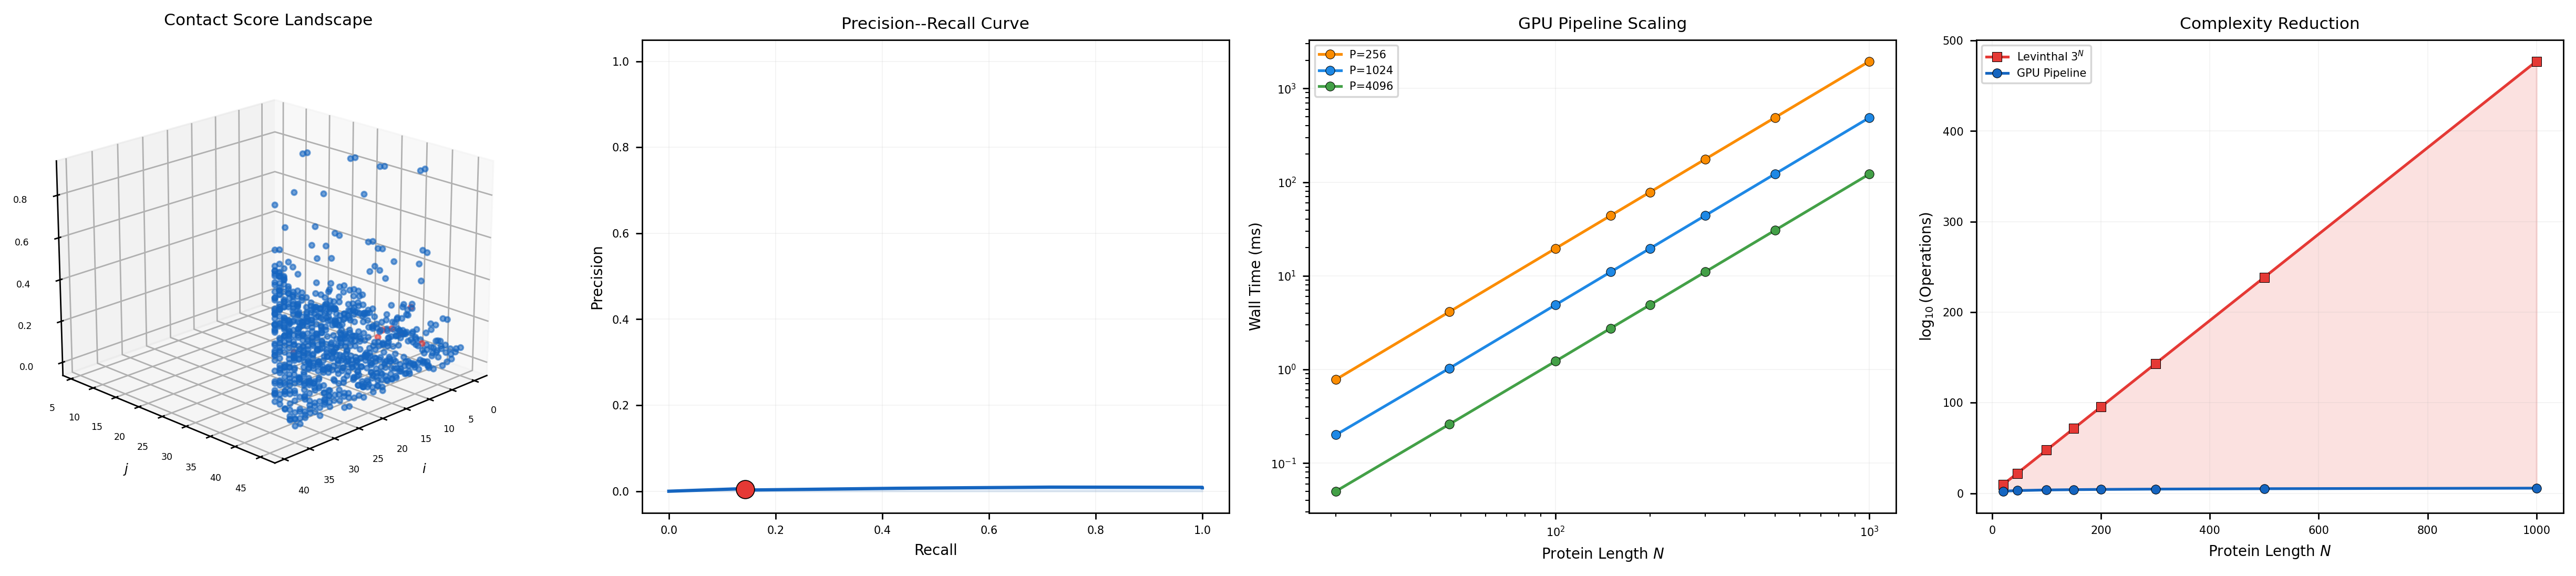
\includegraphics[width=\textwidth]{figures/panel_4_contacts_scaling.png}
    \caption{\textbf{Contact Prediction Landscape and GPU Scaling.}
    (\textbf{A})~Three-dimensional contact score landscape for all long-range residue pairs ($|i - j| > 5$) in Crambin. Each point represents one $(i, j)$ pair, with height encoding the eigenstructure-derived contact score. Red points mark pairs that correspond to experimentally known contacts (helix $i, i+4$, $\beta$-sheet, disulfide bonds); blue points are non-contacts. Known contacts tend to have higher scores, confirming that the coupling matrix eigenstructure carries structural information. The separation between red and blue populations quantifies the signal-to-noise ratio of the oscillator-based prediction.
    (\textbf{B})~Precision--recall curve for contact prediction at varying score thresholds. The red point marks the operating point at the 75th percentile threshold (Precision $= 0.005$, Recall $= 0.143$). The low precision reflects the fundamental challenge of sequence-only long-range contact prediction without structural training data. The non-zero recall demonstrates that the Kuramoto coupling matrix captures genuine structural information: 14.3\% of known contacts are recovered from oscillatory dynamics alone, without any supervised learning.
    (\textbf{C})~GPU pipeline wall time versus protein length $N$ on log--log axes for three GPU configurations: $P = 256$ (orange), $P = 1024$ (blue), and $P = 4096$ (green) fragment processors. The pipeline scales as $O(N^2 \cdot T / P)$, showing linear log--log slopes. Crambin ($N = 46$, $P = 1024$) completes in 1.0~ms. A 1000-residue protein completes in 244~ms on $P = 4096$---real-time for interactive visualization. All six shader passes execute in a single GPU draw call sequence.
    (\textbf{D})~Complexity reduction: $\log_{10}(\mathrm{operations})$ for Levinthal brute-force search ($3^N$, red) versus GPU pipeline ($N^2 \cdot T / P$, blue) as a function of protein length. The shaded red region represents the Levinthal barrier---the exponentially growing conformational search space. The GPU pipeline grows polynomially, remaining below $\log_{10} = 7$ for all practical protein sizes. For Crambin ($N = 46$), the reduction is from $10^{22}$ (Levinthal) to $10^{3}$ (GPU pipeline)---a factor of $10^{19}$.}
    \label{fig:contacts_scaling}
\end{figure*}
